\begin{appendices}
%Material that is complementary to the main body of the report can be included in an appendix. For externally sponsored students, if a report has been submitted to the sponsor during the year of the review, the report should be included in the appendix (a copy of the report can be supplied by the PGR coordinator). The appendix should include a list of training courses (including dates, duration, etc.) taken by the student during the year and other relevant research activities such as given seminars, attendance and presentations to conferences, etc. The appendix could also include material that is supplementary to the main body of the report such as: description of data sets, detailed experimental results, papers that have been submitted or published, etc.

\chapter{Training Courses}
\begin{itemize}
\item Computer Science PGR Introductory Seminar 5 Dates
\item Tradition of Critique Lecture series, Monday 29th September - Monday 8th December (18:00 - 20:00)
\item Graduate School: 
	\begin{itemize}	
		\item Nature of the doctorate and the supervision process, 15th November 2016 (9:30 - 12:00)
		\item Presentation skills for researchers (all disciplines), 27th Jan 2017 (9:30 - 15:30)
		\item Planning your research, 20th Feb 2017 (9:30 - 13:00)
		\item Getting into the habit of writing, 23th Feb 2017 (9:30 - 12:30)
	\end{itemize}
\item Midland Graduate School 2017 from 9-13 April in Leicester. Attended courses on Denotational Semantics, Naïve Type Theory and Testing with Theorem Provers.
\end{itemize}

\chapter{Questions \& Answers}
\label{chap:qa}

TODO: update and adopt to 2nd year

In this chapter I give answers to anticipated questions and objections about my research direction and vision of doing pure functional ABS \footnote{They are not always posed in a dead-serious way but as it is a quite controversial topic - ABS should be done object-orientated after all huh? - I think it is appropriate. Also some objections were raised in exactly this way.}.

\paragraph{So you had this hypothesis, that pure functional programming and dependent types lead to simulation software which is more likely correct and is easier to verify and validate, right from the beginning?}
Not at all. I even had no deep knowledge of functional programming at the start of my PhD, I've just worked through the 1st edition of Grahams book "Programming in Haskell" and that's it. I had no clear understanding of purity, side-effects and Monads and I didn't know a bit about functional reactive programming. I knew that something like Dependent Types exist because Thorsten (2nd Supervisor) has sent me an email before the start of my PhD in which he pointed at Agda, so I started reading a bit about intuitionistic / constructivistic math, tried out a little bit of Agda but quickly gave up because it was way too far away (without really having mastered pure functional programming in Haskell, I believe it is nearly impossible / too difficult / makes no sense going into dependent types).
So in the beginning there was pure \textit{curiosity} about functional programming in combination with ABS because I knew nothing of FP at all and wanted to understand it (after getting bored by OO) and applying FP to ABS seemed so crazy (because everyone claims OO to be 'natural' for it) that it must be an extremely interesting challenge. I guess this is very often the case with research: there is 'just' curiosity in the beginning and then during the research process a hypothesis falls into place.


\chapter{Update-Strategies}
TODO: write short explanation of this paper: tries to develop foundational technical vocabulary for ABS.

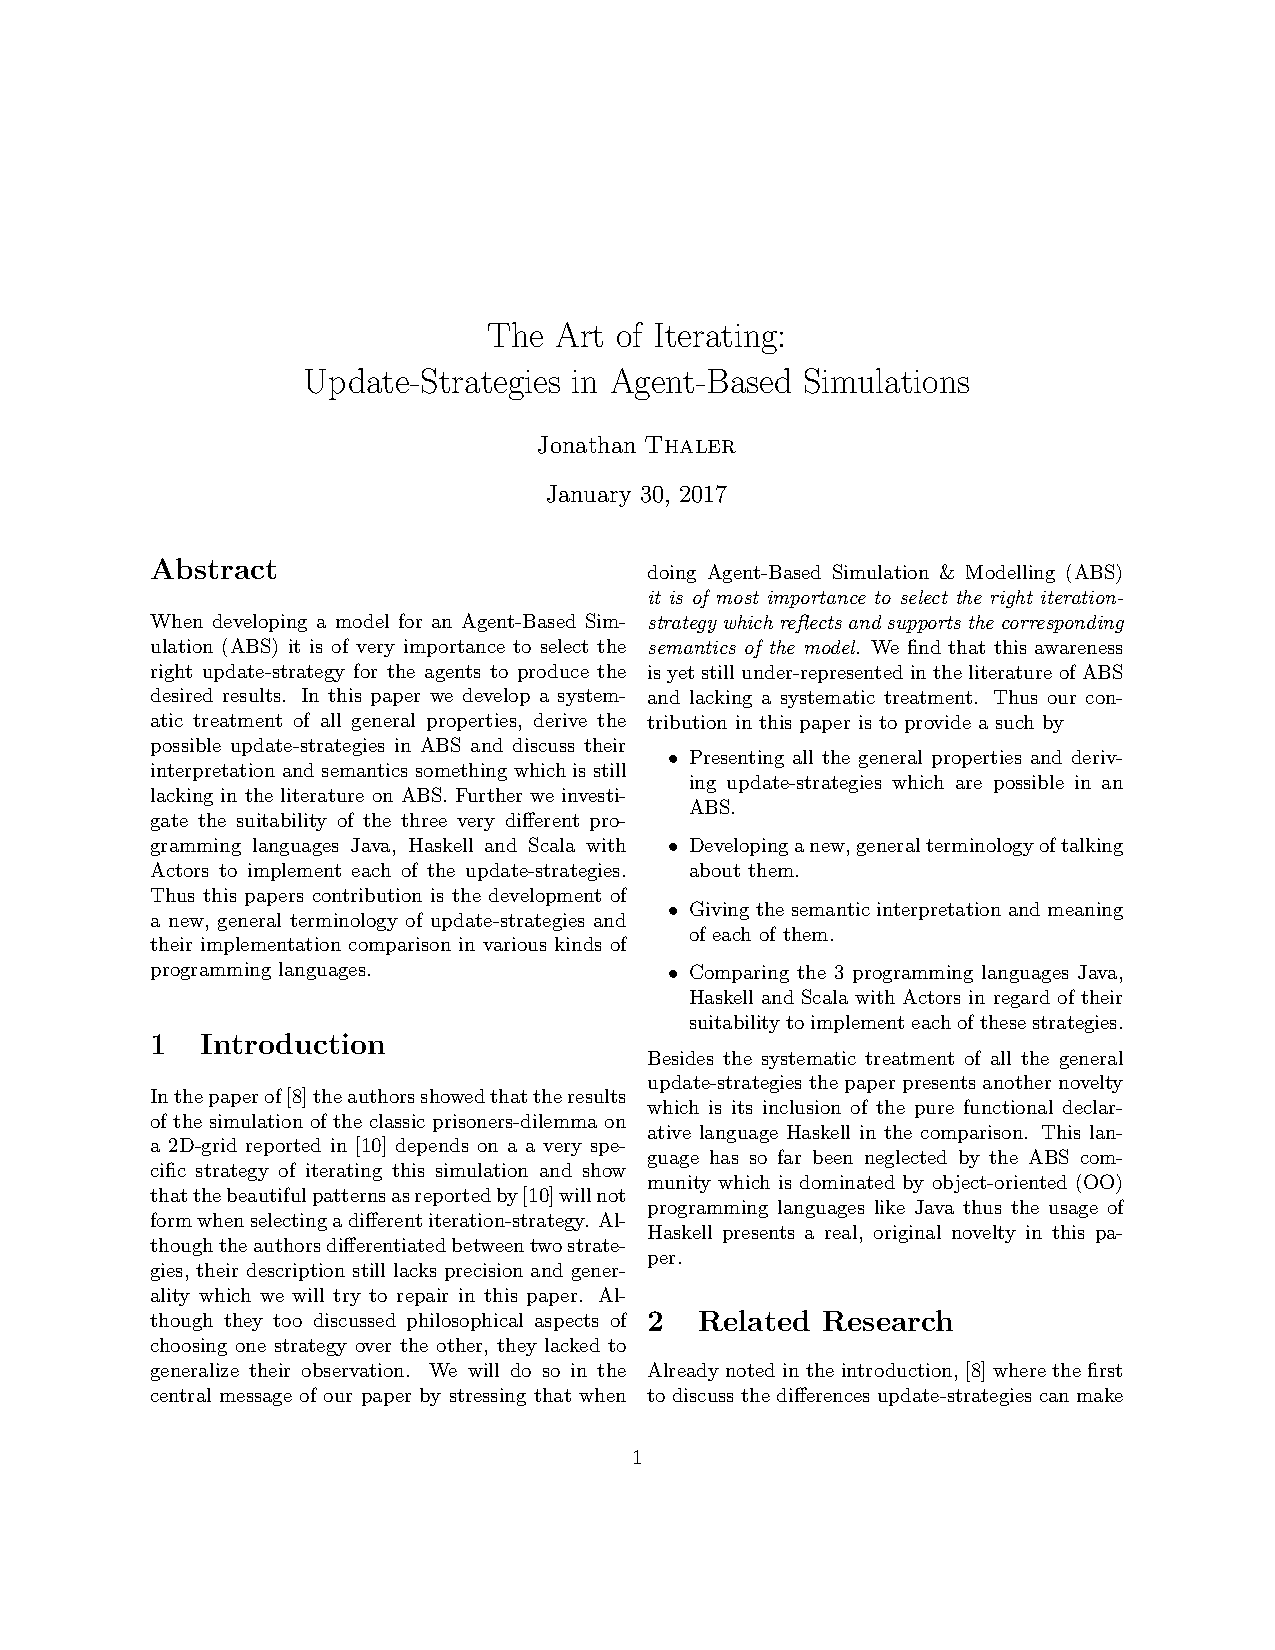
\includepdf[pages=-]{./pdf/iteratingABM.pdf}

\chapter{Programming-paradigms in ABS}
TODO: write short explanation of this paper. emphasize that it was not published but originally part of the update-strategies paper which was then split because of two different things mixed up.

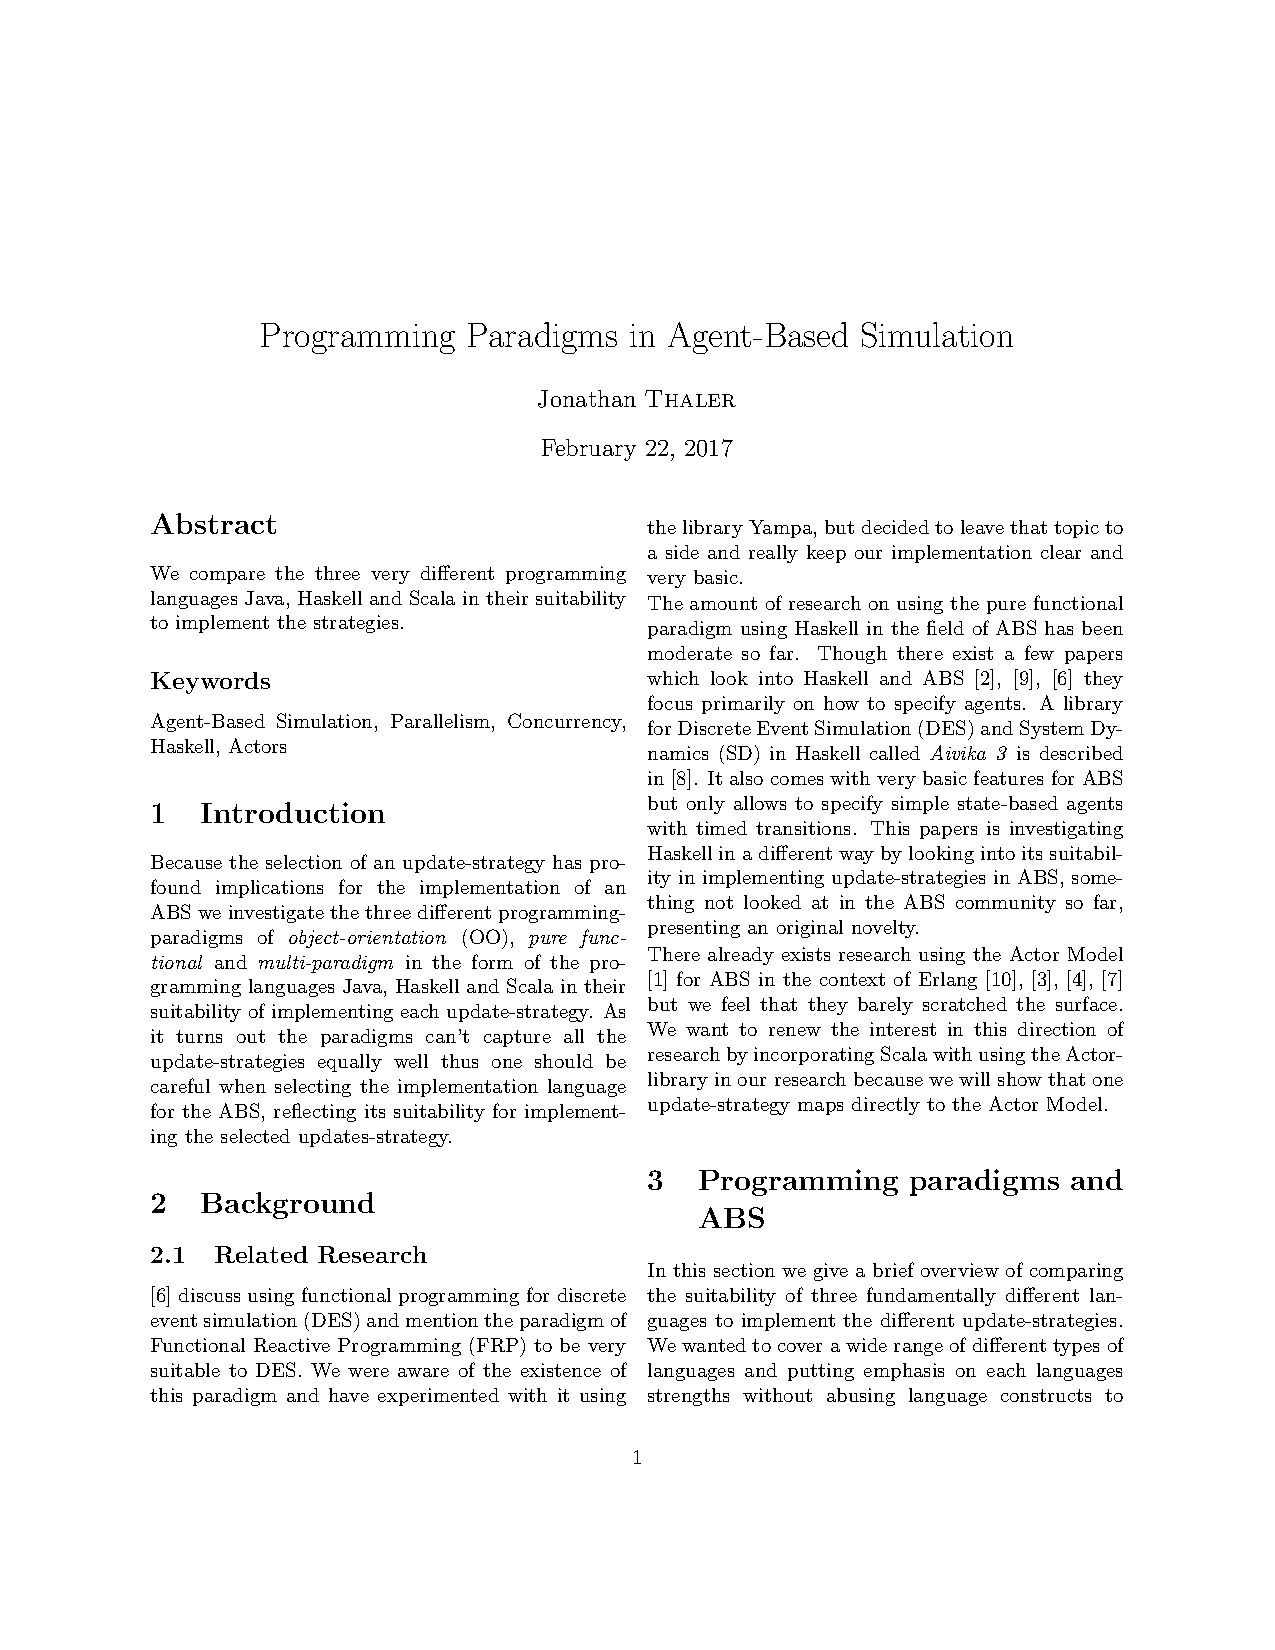
\includepdf[pages=-]{./pdf/programmingParadigmsABS.pdf}

\chapter{Recursive ABS}
TODO: write short explanation of this paper. not published but interesting idea but not enough time to pursue. also why stopped working: don't have the right model in which it serves as a killer-features. still we are convinced that it proves one of the major benefits of FrABS: recursion is easy to implement because the language is built on it and due to the lack of side-effects.

TODO: include, need little bit of refinement: put in the pictures of dynamics

\end{appendices}